The exponential growth of data-intensive applications is pushing the limits of computational hardware. With Moore's Law drawing to a close as silicon transistors reach their physical limits, monolithic chip solutions are fundamentally limited by their ability to scale. Rather than relying on continued miniaturization, the future of computing lies in \emph{parallel architectures} and \emph{heterogeneous integration} to meet the growing demands for performance, yield, and diversified functionality~\cite{iyerHeterogeneousIntegrationPerformance2016}. In modern hyperscale computing infrastructures, such as data centers and high-performance computing systems, the interconnects among heterogeneous computing resources have become integral to the overall system performance, as efficient data movement is critical to avoid data-starved processing units (PUs). Notably, with the rise of large machine learning models comprising billions to trillions of parameters, PUs spatially separated by up to kilometers need to communicate\textemdash{}a distance scale at which electrical signaling over metal wires consumes excessive energy due to distance-dependent losses. A prevailing solution to this challenge is to leverage the properties of light to send data with distance-agnostic losses and high parallelism through optical interconnects~\cite{millerRationaleChallengesOptical2000}. While a significant amount of research exists in using exotic material platforms for realizing specialized optoelectronic devices, the most elegant solution is to leverage the mature, scalable, and cost-effective precision tooling, developed over decades for the electronics industry, to implement optical transceivers in silicon\textemdash{}the motivation that sparked the field of silicon photonics (SiPh)~\cite{sorefPresentFutureSilicon2006}.

\begin{wrapfigure}{r}{0.4\textwidth}
    \vspace{-1em}
    \begin{center}
        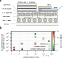
\includegraphics[width=\linewidth]{../../6_figures/rs_fig_1_empho.png}
    \end{center}
    \caption{(a)~FOM comparison between pluggable, existing CPO, and my research, showing key enablers of FOM leaps toward future goal. Data sources given in~\cite{wangCoDesignedSiliconPhotonics2024}. (b)~Illustrative integration stack with pluggable optics. (c)~Illustrative integration stack with CPO and our 96\,Tbps MCP prototype. (d)~Envisioned compute node with embedded photonics, where optical modulators are directly driven by electrical I/Os of processor or memory chips.}
    \label{fig:embedded_photonics}
    \vspace{-3em}
\end{wrapfigure}

After modest initial growth, SiPh has finally seen in the past decade the promise of large-scale integration with thousands to millions of optical components on a single chip~\cite{shekharRoadmappingNextGeneration2024}, following the maturation of 300\,mm SiPh-wafer foundry offerings. The move from individual devices to complex circuits opens up a wealth of interdisciplinary research opportunities at the intersection of photonics, electronics, and computing systems. Over the course of my \myDegree{} and postdoc, I have made significant contributions to diverse yet synergistic areas of SiPh, including electronic-photonic design automation (EPDA)~\cite{wuCompactModelingCircuitlevel2017,zhangCompactModelingSilicon2017,jamesFlexibleProcessAwareCompact2022,jamesProcessVariationAwareCompact2023a}, variation characterization and mitigation~\cite{wuPairingMicroringbasedSilicon2018,wangEnergyefficientChannelAlignment2018,wangTamingEmergingDevices2019,wangBidirectionalTuningMicroringbased2019,wangCharacterizationApplicationsSpatial2020,wangEnergyEfficiencyYield2021}, broadband filters and dispersion engineering~\cite{wangDispersionEngineeredFabricationRobustSOI2023,wangIntegratedCompactTunable2023,parsonsOFC25}, ultra-scalable link architectures~\cite{wangScalableArchitectureSubpJ2023,novickHighbandwidthDensitySilicon2023}, automated link control~\cite{wangAutomatedTuningRingAssisted2024,wangInterleaverTuning,wangOFC25}, channel-dependent optimization~\cite{novickIntegratedPhotonicResonant2024,gopalEqualization2024}, network-application co-optimization~\cite{wangTaskMappingAssistedLaser2019,wangTrafficAdaptivePowerReconfiguration2021,michelogiannakisEfficientIntraRackResource2023,wuWavelengthReconfigurableTransceiver2024,wuFlexibleSiliconPhotonic2024}, and photonics-enabled computing and data processing~\cite{naumanOFC25,zypmanDSP}.

Most notably, my postdoctoral research at \mySchoolShort{} made essential contributions to the first demonstration of a hybrid 2.5D/3D integration of photonic input/output (I/O) chiplets with
flip-chip bonded electronic drivers and a state-of-the-art field-programmable gate array (FPGA)~\cite{wangSiliconPhotonicsChip2024,wangCoDesignedSiliconPhotonics2024,RovinskiISCAS25}. The prototype demonstrated unprecedented shoreline bandwidth density and energy efficiency leveraging Kerr comb\textendash{}driven dense wavelength-division multiplexing (DWDM) and advanced packaging to send/receive massively parallel data streams right at the edge of the processor chip, advancing the link figure of merit (FOM) by two orders of magnitude compared to existing co-packaged optics (CPO) solutions (Fig.~\ref{fig:embedded_photonics}a). These significant results have also substantially contributed to the winning of several subsequent research grants from both government and industry, and led to extensive collaborations with leading industrial partners and academic institutions to refine system prototypes. An overview of this work is presented in the next section alongside future research directions for redefining chip-to-chip connectivity. The subsequent section envisages applications of photonics where computing and signal processing functionalities are integrated within data movement, seeking a paradigm shift of computing systems. Finally, I provide an overview of ecosystem, funding, and collaborations required to realize these visions and a pathway to fulfilling these requirements leveraging my expertise, experience, and network.

\section*{Transforming Chip-to-Chip Connectivity}

A major connectivity bottleneck faced by today's computing clusters is the system-wide link bandwidth discrepancy. As data needs to travel longer distances, the available bandwidth at higher levels of the network hierarchy gradually drops by up to two orders of magnitude to avoid the prohibitive energy required for long-distance electrical signaling. Conventional pluggable optical transceivers (Fig.~\ref{fig:embedded_photonics}b) only extend the reach of the signals, but are fundamentally limited by the excessive power and area required for EO/OE conversion, primarily due to the long electrical traces on-board and the need for high data rates per lane.

As part of the DARPA PIPES program, I spearheaded the photonics design for a photonic I/O chiplet that aims to substantially improve the link FOM, defined as the bandwidth density\textendash{}energy efficiency product [Gbps/mm \texttimes{} (pJ/b)$^{-1}$] (Fig.~\ref{fig:embedded_photonics}a). The link architecture uniquely leverages chip-scale microresonator-based Kerr frequency combs, which are capable of generating hundreds of evenly-spaced low-noise wavelength channels from a single continuous-wave (CW) laser source with high efficiency. This allows achieving a high aggregate data rate with massive wavelength parallelism at a modest data rate per channel\textemdash{}a key enabler of high energy efficiency. Each photonic chiplet, measuring 8.1\,mm \texttimes{} 8.6\,mm, densely integrates over \num{2000} microresonator modulators and filters to deliver a bidirectional bandwidth greater than 32\,Tbps with a 4\,Tbps/mm shoreline bandwidth density. Multi-chip package (MCP) prototypes (Fig.~\ref{fig:embedded_photonics}c) were also developed in collaboration with Intel and Cornell University. Each MCP comprises three electronic driver chiplets fabricated in Intel's 22\,nm process, flip-chip bonded to three photonic transceiver chiplets, and further integrated with an Intel Stratix 10 FPGA using Intel's Embedded Multi-Die Interconnect Bridge (EMIB) technology. This MCP prototype is the first to demonstrate a hybrid 2.5D/3D\textendash{}integrated CPO solution promising of a 96\,Tbps bidirectional bandwidth at a sub-pJ/b energy efficiency. As Fig.~\ref{fig:embedded_photonics}a shows, these results represent a two-order-of-magnitude improvement in the link FOM compared to state-of-the-art CPO solutions, and a \num{1000}\texttimes{} improvement over the best-in-class pluggable transceivers. These results have led the successful transition of the DARPA PIPES program into Phase 3, and substantially contributed to the winning of an SRC JUMP 2.0 grant and a Samsung GRO grant. In these subsequent projects, I have worked closely with leading industrial companies (Intel, Samsung, and Applied Materials), academic institutions (Cornell, MIT, and UIUC), and foundry partners (AIM Photonics and GlobalFoundries) to push the limits of interconnect bandwidth density and energy efficiency through electronic-photonic co-design and heterogeneous integration. A preliminary link budget analysis based on measured devices has shown great promise for another order of magnitude improvement in the link FOM achievable through on-chip laser integration and wafer-scale substrate undercut, marking a significant leap toward the goal in Fig.~\ref{fig:embedded_photonics}a.

\begin{wrapfigure}{l}{0.39\textwidth}
    \vspace{-1em}
    \begin{center}
        \includegraphics[width=\linewidth]{../../6_figures/rs_fig_2_3dpho.png}
    \end{center}
    \caption{(a) Illustrative multi-chip system enabled by dense 3D optical connectivity. (b) Planned prototype of the 3D optical routing assembly with a 10 \texttimes{} 10 array.}
    \label{fig:3d_photonics}
    \vspace{-0.5em}
\end{wrapfigure}

An exciting future extension comes from the deeper integration of photonic I/O with real-world compute/memory resources. As we demonstrated in this work a truly CMOS-compatible driving voltage (<\,0.8\,V) for the microresonator modulators and a pathway to further reduce it below 0.4\,V, I envision a compute node architecture, as shown in Fig.~\ref{fig:embedded_photonics}d, where the processor and memory chips are 3D-integrated with the photonic I/O and directly drives the modulators. This architecture eliminates the need for dedicated serializer/deserializer (SerDes) circuitry and embraces a better match between the data rate of the processor/memory and the optical channel. While in-package resources communicate through low-loss waveguides and off-package data goes through optical fibers, the distance-agnostic nature of optical communication blurs the boundary of nodes and allows for pooling of spatially-distanced resources with comparable latency and energy consumption. This would prove particularly impactful to the system-level deployment of large-scale parallel computing workloads as data locality is no longer a concern.

Looking further ahead, I aim to explore a new paradigm of chip-to-chip connectivity that lifts the restrictions of today's planar optical routing. Despite strong push in link-level performance, the available connectivity between chips is still fundamentally limited by one-dimensional (shoreline) and two-dimensional (areal) chip footprints due to the planar nature of photonic circuits and fiber array sizing. To enable the connectivity scaling, I envision a dense 3D optical system architecture, as illustrated in Fig.~\ref{fig:3d_photonics}a. It enables any-to-any interconnections from waveguide arrays on an active chip to those on another active chip via an interposer-like routing chip, where data stays in the optical domain throughout. The active chips can be integrated with the routing chip via metal-metal hybrid bonding. This approach permits high-density electrical connections between chips for power delivery and control signaling, while
additionally provides high alignment accuracy (<\,200\,nm) and robust mechanical stability for minimizing optical losses due to misalignment. The conceptual design of such a system, which I jointly conceived with my collaborators at \mySchoolShort{},
was well received at the 2023 DARPA ERI Summit. Fig.~\ref{fig:3d_photonics}b shows the plan for a small-scale prototype of the 3D optical routing assembly with a 10 \texttimes{} 10 array of vertical light paths. Upon successful demonstration of this proof-of-concept, the long-term goal is to scale up the connectivity beyond 1000 \texttimes{} 1000 at a drastically denser pitch, ultimately allowing for the integration with heterogeneous computing resources for real-world evaluation. This would open up numerous collaboration opportunities across the system stack, including device, packaging, integration, system architecture, and design automation, to realize the next generation of integrated photonic systems with unprecedented density, efficiency, and connectivity.

\section*{Computing within Data Movement}

With SiPh processes reaching reasonable maturity, various novel applications beyond data communication are emerging. A particular category of applications breaks the traditional boundary between computation and communication regimes by leveraging the analog nature of optical signals to encode and manipulate data within the link paths. Notable architectures include Mach-Zehnder interferometer (MZI) meshes~\cite{shenDeepLearningCoherent2017} and microring weight banks~\cite{taitMicroringWeightBanks2016}, both of which have shown promise in accelerating vector-vector and matrix-vector multiplication operations for AI/machine learning computation. However, these architectures encode the analog weight parameters (the multiplicands) in optical phase or intensity, which are sensitive to fabrication/environmental variations, require complex calibration and control, and are typically limited in scalability and bits precision. Moreover, the digital-to-analog and analog-to-digital conversions at the input/output of these architectures are implemented in electronics, which introduce bottlenecks in the overall system performance and energy efficiency.



\begin{wrapfigure}{r}{0.46\textwidth}
    \vspace{-1em}
    \begin{center}
        \includegraphics[width=\linewidth]{../../6_figures/rs_fig_3_comppho.png}
    \end{center}
    \caption{Illustration of the photonics-enabled data processing architecture for achieving full-digital-precision MAC operations leveraging comb-driven DWDM and photonic ADC.}
    \label{fig:pho_computing}
    \vspace{-0.5em}
\end{wrapfigure}

To address these challenges, a similar architecture to the ultra-broadband DWDM transceivers described earlier can be used, leveraging the manifold wavelengths provided by the comb source. As shown in Fig.~\ref{fig:pho_computing}, this architecture encodes each bit place of the multiplicate-and-accumulate (MAC) result as an analog light intensity and counts the number of 1's through a photonic analog-to-digital converter (ADC). Most uniquely, the architecture directly interfaces with the logic die of the memory chip, taking digital representations of the multipliers/multiplicands and the MAC result as input and output, respectively. Bits precision is determined by the number of parallel wavelengths, and thus takes the best advantage of the comb source. As each wavelength is modulated either on or off, the architecture is inherently more robust to fabrication variations and environmental perturbations. A hardware validation of this architecture is submitted to OFC'25, which demonstrates the efficacy of reusing the DWDM link architecture for data processing functionalities.

As silicon photonics for data communication is beginning to shift from an academic to a commercial field, much like microelectronic integrated circuits in the 1980s, photonics-enabled computing within data movement is seeing a rapid growth of attention, and will make an essential pillar of my future research agenda. Along this line, I am actively exploring the potential of integrating photonic data processing with not only DWDM, but also other architectures such as mode division multiplexing (MDM). Building on my prior experience in advanced packaging and heterogeneous integration, the ultimate goal is to develop a combined photonic I/O\textendash{}processor chip embedded within the package where data is stored/generated. In this architecture, data requesters will fetch computation results directly, rather than raw data. This approach minimizes data movement, reduces latency, and improves energy efficiency by performing computations where data resides and avoiding unnecessary EO/OE conversions between communication and computation. The envisioned architecture initiates a shift in computing paradigm and also finds applications in emerging fields beyond AI/machine learning, such as using photonic data links as the back plane of large-scale antenna arrays and perform signal processing while data is in motion.

\section*{Ecosystem, Funding, and Collaborations}

To achieve the ultimate goal of large-scale integrated photonics involves leveraging the ``fabless'' silicon photonics ecosystem in which chips are fabricated on 300\,mm wafers in billion-dollar state-of-the-art micro-electronics foundries with capabilities far beyond those of university cleanrooms. Over the past few years, I have participated in nine ``tape-outs'' with three commercial foundries in the U.S., including a dedicated 300\,mm wafer run with AIM Photonics in November 2023 where I co-led the design and aggregation. I have also built my own connection with a commercial foundry in Taiwan, which started offering SiPh multi-project wafer (MPW) and custom full-wafer runs to universities after a constructive dialogue with their representatives at OFC'23. Throughout these experiences, I have developed the necessary knowledge and network to lead a research group that leverages the fabless model. Moreover, my \myDegree{} work in compact modeling partially laid the foundation of EPDA, which equipped me with the skills and mindset to contribute to the development of an ``open'' process design kit (PDK) for the mutual benefit of the SiPh community.

During my postdoctoral research, I have led the design and reporting efforts on projects funded by DARPA and ARPA-E, both of which successfully progressed to Phase 3. Notably, I have had the opportunity to attend various
DARPA review sessions and speak directly with program managers, providing an inside perspective on the
critical elements of successful proposals and criteria for advancement along program phases. I have also been deeply involved in the CUbiC Center under the SRC JUMP 2.0 program, where I frequently interact with PIs from 15 leading universities and liaisons from 15 commercial and defense electronics industry sponsors, providing me with a solid foundation for future relationships. Furthermore, I have gained abundant experience in applying for research grants by contributing to the writing of more than ten proposals over the past two years, including four winning ones from both government and industry sources. Recently, I have been actively involved in the preparation of two large-scale proposals under the CHIPS Act, aiming to push the limits of photonic I/O packaging and build a digital twin for its design and integration process. I believe these extensive experiences will provide me with a competitive edge in acquiring external funding through a deep understanding of the key characteristics of successfully-funded proposals.

My close relationships across academia will provide immediate research avenues that expand on previous work and enable entirely new directions. In particular, my ongoing collaborative relationships
with Profs. Keren Bergman, Michal Lipson, and Alexander Gaeta at \mySchoolShort{} have been highly fruitful, with many additional directions jointly identified for future work. At \appSchoolDeptShort{}, I will make the best use of my existing network to give my research group a head start. I additionally envision the opportunity for new collaborations with the current faculty at \appSchoolShort{}, including:
\begin{enumerate*}[label=(\roman*)]
    \appCollab{}
\end{enumerate*}
I am excited to contribute my experience
and enthusiasm to your esteemed institution, keenly anticipating the chance to work with a community that resonates my commitment to making a meaningful impact on the future of computing.